\chapter{Theoretical and experimental background} % (fold)
\label{cha:theoretical_background}
%%%%%%%%%%%%%%%%%%%%%%%%%%%%%%%%%%%%%%%%%%%%%%%%%%%%%%%%%%%%%%%%%%%%%%%%%%%%%%%%%%%%%%%%%%%%%%%%%%%%%%%%%%%%%%%%%%
%%%%%%%%%%%%%%%%%%%%%%%%%%%%%%%%%%%%%%%%%%%%%%%%%%%%%%%%%%%%%%%%%%%%%%%%%%%%%%%%%%%%%%%%%%%%%%%%%%%%%%%%%%%%%%%%%%
%%%%%%%%%%%%%%%%%%%%%%%%%%%%%%%%%%%%%%%%%%%%%%%%%%%%%%%%%%%%%%%%%%%%%%%%%%%%%%%%%%%%%%%%%%%%%%%%%%%%%%%%%%%%%%%%%%
%%%%%%%%%%%%%%%%%%%%%%%%%%%%%%%%%%%%%%%%%%%%%%%%%%%%%%%%%%%%%%%%%%%%%%%%%%%%%%%%%%%%%%%%%%%%%%%%%%%%%%%%%%%%%%%%%%
%%%%%%%%%%%%%%%%%%%%%%%%%%%%%%%%%%%%%%%%%%%%%%%%%%%%%%%%%%%%%%%%%%%%%%%%%%%%%%%%%%%%%%%%%%%%%%%%%%%%%%%%%%%%%%%%%%
\section{Attosecond dynamics} % (fold)
\label{sec:attosecond_dynamics}

Understanding and imaging motion on fast time scales has been of interest for more than a century. In 1878, Eadweard Muybridge invented high speed photography to find out if all of a horse's feet leave the ground at a full gallop \cite{muybridge1978}. Since then, high speed photography has reached time scales of $\sim10^{-5}$s, a long ways off of the attosecond ($10^{-18}$s) time scale of electron motion. On attosecond time scales, only electrons in atoms and molecules display significant motion (see Fig.~\ref{fig:time_scales}) rendering electronic or mechanical shutters, from traditional photography, useless. Additionally, the electrons being imaged are quantum objects further complicating the imaging process. Before we go into the methods used for imaging electron motion, lets dive into what we mean when we say a quantum object is moving. 

For a time independent system, such as an atom or molecule in vacuum, there exists a set of stationary states that are eigenfunctions of the system's Hamiltonian (for details see Sec.~\ref{sec:TDSE}). In the case of an atom or molecule, these stationary states are the bound or continuum states which we will call $\ket{\psi_j(\mathbf{r})}$. These states depend on space, and evolve in time like $e^{iE_j t}$ where $E_j$ is the energy of the $j$th stationary state, $i=\sqrt{-1}$ is the imaginary number, and $t$ is time. This shows that only the phase of the state is changing in time. As the global phase of a wavefunction is not observable, an electron occupying a single stationary state displays no motion. 

For attosecond motion to occur, either the system's Hamiltonian must become time dependent, e.g.\ by introducing a laser pulse, and/or multiple stationary states must be populated forming a superposition. The former is often required to image the motion of electrons, but the latter is simpler to understand. We will, therefore, start with the motion produced by an electron in a superposition of more than one stationary state. In principle, one or more of the states could be continuum states, but for simplicity we restrict ourselves to bound states only in the following discussion. The resulting electronic wavefuction can be written as
\begin{equation}
\label{eq:atto_dynamics}
    \ket{\Psi(\mathbf{r},t)} = \sum_{j=0}^{N-1} a_j e^{i(\phi_j +E_jt)}\ket{\psi_j(\mathbf{r})}
\end{equation}
where $a_j$ is a non-negative real number, $\phi_j$ is a phase, $E_j$ is the energy of the state, and the superposition contains $N$ total states each labeled by the subscript $j$. The global phase can be accounted for by removing the time dependent phase of the ground state by setting $E_0=0$. The relative phases of the excited states ($j>0$) changes in time like $(E_j-E_0)t$ resulting in dynamics if $E_j\ne E_0$. For a two state system, the dynamics will be periodic with a period of $T=2\pi/|E_1- E_0|$. Fig.~\ref{fig:he_dynamics} shows the dynamics of the wavefunction for a helium atom in a $1s-2p_+$ superposition as it rotates with a period of approximately 200 attosecond.

\begin{figure}[!ht]
\centering
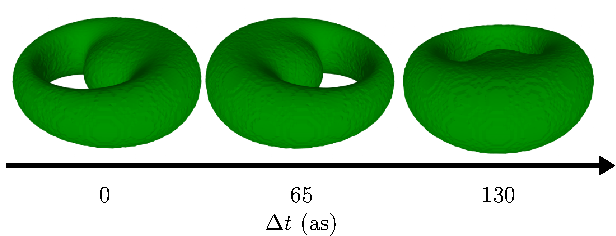
\includegraphics[width=\columnwidth]{figs/background/dynamics.pdf}
\caption{\label{fig:he_dynamics} An isosurface of the wavefunction of a helium atom in a $1s-2p_+$ superposition ($|r\Psi|$) undergoing attosecond motion. (Figure from \cite{venzke2021_wave})
}
\end{figure}

Adding additional states to the superposition allows for arbitrarily complicated field free dynamics to occur. In order to ``image'' the wavepacket, all of the values for $a_j$ and $\phi_j$ must be obtained at some time $t_0$ with the restrictions that $a_0 = \sqrt{1-\sum_{j=1}^{N-1} a_j^2}$ and $\phi_0=0$ to enforce normalization and removing the global phase, respectively. Then using Eq.~\ref{eq:atto_dynamics}, the time dependence of the system is known. A method for imaging simple superpositions is presented in Sec.~\ref{sec:wavefunction_reconstruction}.

When the system's Hamiltonian becomes time dependent, however, the above approach does not capture the dynamics completely. If the time dependent operator is weak relative to the time independent operators, the dynamics maybe captured by allowing $a_j$ and $\phi_j$ to become time dependent quantities. When effect of the time dependent operator becomes comparable or larger than the independent operators, the stationary states, $\ket{\psi_j(\mathbf{r})}$, may no longer be a good basis to describe the system. Imaging the dynamics of such a system requires techniques beyond the scope of this thesis.
% section attosecond_dynamics (end)

%%%%%%%%%%%%%%%%%%%%%%%%%%%%%%%%%%%%%%%%%%%%%%%%%%%%%%%%%%%%%%%%%%%%%%%%%%%%%%%%%%%%%%%%%%%%%%%%%%%%%%%%%%%%%%%%%%
%%%%%%%%%%%%%%%%%%%%%%%%%%%%%%%%%%%%%%%%%%%%%%%%%%%%%%%%%%%%%%%%%%%%%%%%%%%%%%%%%%%%%%%%%%%%%%%%%%%%%%%%%%%%%%%%%%
%%%%%%%%%%%%%%%%%%%%%%%%%%%%%%%%%%%%%%%%%%%%%%%%%%%%%%%%%%%%%%%%%%%%%%%%%%%%%%%%%%%%%%%%%%%%%%%%%%%%%%%%%%%%%%%%%%
%%%%%%%%%%%%%%%%%%%%%%%%%%%%%%%%%%%%%%%%%%%%%%%%%%%%%%%%%%%%%%%%%%%%%%%%%%%%%%%%%%%%%%%%%%%%%%%%%%%%%%%%%%%%%%%%%%
%%%%%%%%%%%%%%%%%%%%%%%%%%%%%%%%%%%%%%%%%%%%%%%%%%%%%%%%%%%%%%%%%%%%%%%%%%%%%%%%%%%%%%%%%%%%%%%%%%%%%%%%%%%%%%%%%%
\section{Pump-probe spectroscopy} % (fold)
\label{sec:pump_probe_spectroscopy}
Pump-probe spectroscopy is a powerful tool for imaging ultrafast processes. The general concept is quite simple. Two isolated ultrashort pulses are produced. The first pulse, known as the probe pulse, prepares the system by starting some dynamical process. Some time after the end of the first pulse, the second (probe) pulse images the target. By delaying the probe pulse with respect to the pump pulse, the impact of the dynamics on a given observable can be observed experimentally. This gives a glimpse at how the system evolves over time. Although conceptually easy to understand, attosecond pump-probe spectroscopy is an extremely difficult experiment to perform for the following reasons. 

In many cases, it is required to have both angle- and/or energy-resolved spectra of the ionized electrons. With the development of experimental techniques, such as velocity map imaging (VMI) \cite{kornilov2010,rouzee2011} or cold target recoil ion momentum spectroscopy (COLTRIMS) \cite{ullrich2003}, the detection of angle-resolved emission of the photoelectron following few-photon ionization of atomic and molecular targets has become possible \cite{ma2013}. 
Additionally, one requires the ability to produce well controlled isolated ultrafast laser pulses. In the recent past, it has become possible to generate isolated attosecond pulses \cite{frank2010}. This has opened the door for the application of pump-probe spectroscopy to attosecond physics. 

In 2001, the first experimental observation of attosecond electron dynamics was made with a pump-probe setup including an few cycle visible light pulse and an attosecond soft-X-ray pulse \cite{hentschel2001}. The bandwidth of attosecond laser pulses allows for both bound and continuum states to be studied \cite{mauritsson2010} and, more recently, charge dynamics in Tryptophan on the sub 4fs time scale have been observed showing that attosecond pump-probe spectroscopy may be applied to complex molecules \cite{larasstiaso2018}. As experimental techniques evolve, the application of attosecond pump-probe experiments will continue to expand. In this thesis, we look at how pump-probe spectroscopy can be used to understand the ionization of electrons in superposition states in Sec.~\ref{sec:generalized_asymmetry_parameters} and reconstruct attosecond electron motion in Sec.~\ref{sec:wavefunction_reconstruction}.
% section pump_prop_spectroscopy (end)

%%%%%%%%%%%%%%%%%%%%%%%%%%%%%%%%%%%%%%%%%%%%%%%%%%%%%%%%%%%%%%%%%%%%%%%%%%%%%%%%%%%%%%%%%%%%%%%%%%%%%%%%%%%%%%%%%%
%%%%%%%%%%%%%%%%%%%%%%%%%%%%%%%%%%%%%%%%%%%%%%%%%%%%%%%%%%%%%%%%%%%%%%%%%%%%%%%%%%%%%%%%%%%%%%%%%%%%%%%%%%%%%%%%%%
%%%%%%%%%%%%%%%%%%%%%%%%%%%%%%%%%%%%%%%%%%%%%%%%%%%%%%%%%%%%%%%%%%%%%%%%%%%%%%%%%%%%%%%%%%%%%%%%%%%%%%%%%%%%%%%%%%
%%%%%%%%%%%%%%%%%%%%%%%%%%%%%%%%%%%%%%%%%%%%%%%%%%%%%%%%%%%%%%%%%%%%%%%%%%%%%%%%%%%%%%%%%%%%%%%%%%%%%%%%%%%%%%%%%%
%%%%%%%%%%%%%%%%%%%%%%%%%%%%%%%%%%%%%%%%%%%%%%%%%%%%%%%%%%%%%%%%%%%%%%%%%%%%%%%%%%%%%%%%%%%%%%%%%%%%%%%%%%%%%%%%%%
\section{Few photon ionization} % (fold)
\label{sec:few_photon_ionization}
Multiphoton ionization was proposed by G\"oppert-Mayer in 1931 \cite{goppertmayer1931}. Thirty years later, two photon ionization was demonstrated experimentally shortly after the advent of the laser \cite{kaiser1961}. As we approach a century since the proposal of multiphoton ionization, research in this area is still progressing. With recent advances in HHG and FEL laser pulse sources in the extreme-ultraviolet (EUV) wavelength regime, studies involving few photon ionization in the perturbative intensity regime have been of both experimental and theoretical interest \cite{nikolopoulos2001,vanderhart2005,shakeshaft2007,pi2010,florescu2011,sato2011,haber2011,florescu2012,ishikawa2012,ishikawa2013,ma2013,rey2014,grum-grzhimailo2015,douguet2016,hofbrucker2017,hofbrucker2018,boll2019,wang2019}. Using tools like VIM and COLTRIMS allows for both the direction and momentum of the ionized electrons to be detected. At a given electron energy, the probability distribution of an electron being ionized in a specific direction is known as a photoelectron angular distributions (PAD). 

PADs contain information containing about the phase and amplitude of the various partial waves produced during the ionization process. These signals have been used to study the competition between resonant and non-resonant two-photon ionization pathways \cite{ishikawa2012,ishikawa2013,ma2013} and between one- and two-photon ionization channels \cite{grum-grzhimailo2015,douguet2016,boll2019}.
These tools are also used to investigate the impacts of many other physical effects, such as a significant circular dichroism via the asymmetry in the forward-backward electron emission from bromocamphor molecules induced by circularly polarized light has been identified  \cite{bowering2001}. Observation of the breakdown of the symmetry in the photoelectron emission of argon has been shown in the region of the Cooper minimum \cite{ilchen2018}, molecular vibrations and chirality have been studied \cite{garcia2013} and other applications range from studies of coherent control \cite{prince2016} to the characterization of ultrashort laser pulses \cite{chelkowski2002}.

Through the contents of Chap.~\ref{cha:imaging_wave_packets_with_photoelectrons} we explore the impacts of few photon ionization using ultrashort pulses (Sec.~\ref{sec:short_pulse_effect}), proposing new asymmetry parameters for understanding few photon ionization of electrons in superpositions  (Sec.~\ref{sec:generalized_asymmetry_parameters}) and how few photon ionization can be used to reconstruct attosecond electron motion (Sec.~\ref{sec:wavefunction_reconstruction}).
% section few_photon_ionization (end)

%%%%%%%%%%%%%%%%%%%%%%%%%%%%%%%%%%%%%%%%%%%%%%%%%%%%%%%%%%%%%%%%%%%%%%%%%%%%%%%%%%%%%%%%%%%%%%%%%%%%%%%%%%%%%%%%%%
%%%%%%%%%%%%%%%%%%%%%%%%%%%%%%%%%%%%%%%%%%%%%%%%%%%%%%%%%%%%%%%%%%%%%%%%%%%%%%%%%%%%%%%%%%%%%%%%%%%%%%%%%%%%%%%%%%
%%%%%%%%%%%%%%%%%%%%%%%%%%%%%%%%%%%%%%%%%%%%%%%%%%%%%%%%%%%%%%%%%%%%%%%%%%%%%%%%%%%%%%%%%%%%%%%%%%%%%%%%%%%%%%%%%%
%%%%%%%%%%%%%%%%%%%%%%%%%%%%%%%%%%%%%%%%%%%%%%%%%%%%%%%%%%%%%%%%%%%%%%%%%%%%%%%%%%%%%%%%%%%%%%%%%%%%%%%%%%%%%%%%%%
%%%%%%%%%%%%%%%%%%%%%%%%%%%%%%%%%%%%%%%%%%%%%%%%%%%%%%%%%%%%%%%%%%%%%%%%%%%%%%%%%%%%%%%%%%%%%%%%%%%%%%%%%%%%%%%%%%
\section{Rydberg state excitations induced by strong fields} % (fold)
\label{sec:rydberg_state_excitations_induce_by_strong_fields}
Excited states in atoms and molecules have played an important role in the understanding of many physical phenomena in strong field physics such as  resonant enhancement in the population of excited states \cite{deboer1992,jones1992}, structures in the energy spectrum \cite{freeman1987,perry1989,agostini1989}, and in energy-resolved angular distributions \cite{rottke1994} of photoelectrons. When excited states become resonant with a one- or multiphoton process from an initial state, the electron can populate the excited state. Depending on the system and laser involved, the population in the excited state can be trapped or it can enhance the probability of another process occurring. The role of excitation was initially observed via resonant enhancement in the population of excited states \cite{deboer1992,jones1992} and structures in the energy spectrum \cite{freeman1987,perry1989,agostini1989} and in energy-resolved angular distributions \cite{rottke1994} of photoelectrons. 

As the laser intensity increases, the ionization potential of an atom shifts into the continuum due to the AC-Stark shift. Additionally, the resonances of highly excited states, known as Rydberg states, follow the same trend. The AC-Stark shifted resonance ($E'$) for highly excited states is therefore approximately 
\begin{equation}
    E' = E + U_p\, ,
\end{equation}
where $E$ is the field-free energy of the excited state, $U_p = I/4\omega^2$ is the ponderomotive energy, $I$ is the peak laser intensity, $\omega$ is the central frequency of the laser, and $E'$ is the energy of the shifted resonance. The initial findings were explained examining the effects of multiphoton absorption becoming resonant with the AC-Stark shifted states.

More recently, significant excitation of atoms has also been observed in the tunneling regime and described by the frustrated tunneling ionization (FTI) model for linearly polarized lasers \cite{nubbemeyer2008}. Similar to the three-step model of HHG, the FTI model starts with the tunnel ionization of an electron. The electron then interacts with the trailing end of the laser pulse which is slowing it down. Finally, the electron is recaptured by the ionic potential ending with a final energy corresponding to that of a Rydberg state. This observation has renewed the general interest in the mechanisms leading to the population of excited Rydberg states during the interaction of an atom with an intense laser pulse (most recently, e.g., in Refs. \cite{chini2014,li2014,li2014b,zimmermann2015,shao2015,camp2015,li2015,fechner2015,bredtmann2016,fushitani2016,lv2016,serebryannikov2016,hart2016,li2016,xiong2016,beaulieu2016,larimian2016,zimmermann2017,bengtsson2017,gao2017,ivanov2017,ilchen2017,mancuso2017,xiong2017,piraux2017}).

The FTI model is semi-classical and provides no predictive power for the angular momentum distribution of the populated excited states. Therefore, recent theoretical studies of the excitation mechanism in linearly polarized strong fields mainly consider the distribution of the population as a function of the principal quantum number of the excited states \cite{li2014,li2014b,zimmermann2017,xiong2017,piraux2017}. It was shown that the modulation of the excitation probability is related to the channel closing effect \cite{krajewska2012,li2014,li2014b,piraux2017}. The latter phenomenon occurs at threshold intensities at which the absorption of one more photon is needed to ionize the atom due to the AC- Stark shift. The interpretation that an increase in excitation can be understood as result of the shift of the first ATI peak below the ionization threshold \cite{li2014,li2014b} is in agreement with the explanation of earlier experimental results (e.g., \cite{freeman1987,jones1992,rottke1994}) via the resonance enhanced population of AC-Stark shifted excited states. 

On the other hand, the literature provides very limited understanding of the angular momentum distribution in the populated Rydberg states by linearly polarized fields. Assuming the initial state has even angular momentum, it has been shown that the populated Rydberg states have angular momentum with the same parity as $N_p-1$, with $N_p$ being the minimum number of photons needed to ionize the AC-shifted ionization potential using Floquet theory for a monochromatic laser field \cite{krajewska2012} and results of numerical calculations for laser pulses with a trapezoidal envelope \cite{piraux2017}. Furthermore, the angular quantum number of the states with the largest population in numerical calculations \cite{li2014,li2014b,piraux2017} agrees well with semiclassical estimations \cite{arbo2008}, initially performed for low-energy angular resolved photoelectron distributions.

For more complex laser set-ups, such as bichromatic circularly polarized laser pulses, almost no work on the population of Rydberg states has been done. Recently, in bicircular fields it has been observed that the probability to ionize an atom is significantly enhanced if the two fields are counter-rotating as compared to co-rotating fields \cite{mancuso2016}.
In that work, the authors propose that the counter-rotating pulse's ionization pathways allow for resonance enhanced ionization while the co-rotating pulse's do not due to selection rules.
However, distributions over the quantum numbers (principal, angular momentum, magnetic) were not presented. Such analysis can shed further light on the role of excited states in the pathways to ionization since excitation in a resonant multiphoton process should rely on the spin-angular momentum selection rules for the absorption of circularly polarized photons.

In this thesis, we examine the excitation of Rydberg states in Chap.~\ref{cha:rydberg_state_excitations}. We study the angular momentum distributions caused by linearly polarized lasers in Sec.~\ref{sec:linear_polarization} and the various mechanisms present in the excitation of Rydberg states by bicircular laser pulses in Sec.~\ref{sec:bi_circular_polarization}.
% section rydberg_state_excitations_induce_by_strong_fields (end)

%%%%%%%%%%%%%%%%%%%%%%%%%%%%%%%%%%%%%%%%%%%%%%%%%%%%%%%%%%%%%%%%%%%%%%%%%%%%%%%%%%%%%%%%%%%%%%%%%%%%%%%%%%%%%%%%%%
%%%%%%%%%%%%%%%%%%%%%%%%%%%%%%%%%%%%%%%%%%%%%%%%%%%%%%%%%%%%%%%%%%%%%%%%%%%%%%%%%%%%%%%%%%%%%%%%%%%%%%%%%%%%%%%%%%
%%%%%%%%%%%%%%%%%%%%%%%%%%%%%%%%%%%%%%%%%%%%%%%%%%%%%%%%%%%%%%%%%%%%%%%%%%%%%%%%%%%%%%%%%%%%%%%%%%%%%%%%%%%%%%%%%%
%%%%%%%%%%%%%%%%%%%%%%%%%%%%%%%%%%%%%%%%%%%%%%%%%%%%%%%%%%%%%%%%%%%%%%%%%%%%%%%%%%%%%%%%%%%%%%%%%%%%%%%%%%%%%%%%%%
%%%%%%%%%%%%%%%%%%%%%%%%%%%%%%%%%%%%%%%%%%%%%%%%%%%%%%%%%%%%%%%%%%%%%%%%%%%%%%%%%%%%%%%%%%%%%%%%%%%%%%%%%%%%%%%%%%
\section{Electron correlation} % (fold)
\label{sec:electron_correlation}

For many effects in ultrafast physics, the single-active electron approximation (SAE), where one electron is allowed to move in an effective potential of all remaining electrons and nuclei, is valid. However, for laser pulses with high energy photons, multiple electrons can interact leading to effects caused by electron correlation. Boll et al.\ recently showed that the SAE approximation breaks down for in the interaction of helium with lasers at high central frequencies \cite{boll2019}.

Electron correlation effects can manifest themselves in many ways. One such example can be found in direct vs.\ autoionizing channels \cite{cirelli2018} where anisotropy and asymmetry parameters have been used to study the impact of the $3s^{-1}np$ resonance in argon. When interacting with an autoionizing resonance, a photon is absorbed by an electron with energy that would allow for ionization and the promotion of a second electron to an excited state. The first electron remains in the resonant state long enough to share its energy via electron correlation with another electron that is excited to a state of higher energy. The first electron is then ionized at a lower energy. 

In addition to autoionizing resonances, two electrons can be ionized by a single photon in a process known as single photon double ionization \cite{maulbetsch1992}. The process proceeds via two main mechanisms, non-sequential double photoionaization (NSDI) and shake-off. In NSDI, the first electron absorbs a high energy photon before it interacts with a second electron. Both electrons are then ionized with similar final energies. The ionized electrons are correlated and have been shown to produce a double slit pattern when double ionizing the H$_2$ molecule \cite{akoury2007}. When even higher photon energies are used, the first electron can be ionized so quickly, that the ionic potential is rapidly  changed and a second electron is ionized with a vary small relative momentum in the shake-off process \cite{carlson1965}.
At even higher photon energies, core electrons can be ionized leaving a hollow atom. A valence electron can then relax into the hole left behind. To conserve energy, a second valence electron is ionized in a process known as the Auger effect originally proposed in 1922 \cite{meitner1922}. 

In order to study these problems in detail, fully correlated multi-electron calculations are required. A solution to the time dependent Schr\"odinger equation (TDSE) in full dimensions requires $3N_e+1$ dimensions where $N_e$ is the number of electrons and the last dimension is time. For time dependent problems, a full solution for two electrons is possible, but requires the use of supercomputer resources \cite{vanroose2006}. The typical approach is to expand the wavefunction in bi-spherical harmonics resulting in two radii that must be discretized to large distances increasing the size of the wavefunction to be stored. In Chap.~\ref{cha:electron_correlation} we discuss our recent developments and first tests of a two-electron code based on hyperspherical harmonics with the goal to potentially remove the need for supercomputers since only a single radius needs to be discretized.
% section electron_correlation (end)

% chapter theoretical_background (end)